\documentclass[12pt]{article}
\usepackage{ctex}
% \usepackage[margin=1.25in]{geometry}
\usepackage[inner=2.0cm,outer=2.0cm,top=2.5cm,bottom=2.5cm]{geometry}
\usepackage{color}
\usepackage{graphicx}
\usepackage{amssymb}
\usepackage{amsmath}
\usepackage{amsthm}
\usepackage{bm}
\usepackage{hyperref}
\usepackage{multirow}
\usepackage{mathtools}
\usepackage{enumerate}

\def \ALC {\mathcal{ALC}}
\def \K {\mathcal{K}}
\def \J {\mathcal{J}}
\def \T {\mathcal{T}}
\def \A {\mathcal{A}}
\def \I {\mathcal{I}}


\newcommand{\homework}[5]{
	\pagestyle{myheadings}
	\thispagestyle{plain}
	\newpage
	\setcounter{page}{1}
	\noindent
	\begin{center}
		\framebox{
			\vbox{\vspace{2mm}
				\hbox to 6.28in { {\bf KRP \hfill #2} }
				\vspace{6mm}
				\hbox to 6.28in { {\Large \hfill #1 \hfill} }
				\vspace{6mm}
				\hbox to 6.28in { {\it Instructor: {\rm #3} \hfill Name: {\rm #4}, StudentId: {\rm #5}}}
				\vspace{2mm}}
		}
	\end{center}
	% \markboth{#4 -- #1}{#4 -- #1}
	\vspace*{4mm}
}


\begin{document}
\large
	%==========================Put your name and id here==========================
	\homework{Homework 4}{Spring 2023}{YiZheng Zhao}{张运吉}{211300063}
    \paragraph{Question 1. $\mathcal{ALC}$-Worlds Algorithm}~{}
    \\

    The role depth of all defined concept name are as follow:
    \begin{equation}
        \begin{aligned}
            \operatorname{rd}(B_0) &= 2, \operatorname{rd}(B_1) = 1, \operatorname{rd}(B_2) = 2, \operatorname{rd}(B_3) = 0 \\
            \operatorname{rd}(B_4) &= 1, \operatorname{rd}(B_5) = 2, \operatorname{rd}(B_6) = 0, \operatorname{rd}(B_7) = 2 \\
            \operatorname{rd}(B_8) &= 2, \operatorname{rd}(B_9) = 1, \operatorname{rd}(B_{10}) = 0 
        \end{aligned} \nonumber
    \end{equation} \par
    Therefore, $i = \operatorname{rd}(B_0) = \max(\operatorname{rd}(B_1), \operatorname{rd}(B_2)) = 2$. 
    \begin{align*}
        \operatorname{Def}_0(\mathcal{T})&=\{ B_3,  B_6, B_{10}\} \\
        \operatorname{Def}_1(\mathcal{T})&=\{ B_1,B_3, B_4, B_6,  B_9, B_{10}\} \\
        \operatorname{Def}_2(\mathcal{T}) & =\{B_0, B_1, B_2,B_3, B_4, B_5, B_6, B_7, B_8, B_9, B_{10}\} 
    \end{align*}
    \begin{itemize}
        \item Successful run. \par
        We guess a set $\tau = \{ B_0, B_1, B_2,B_3, B_4, B_5, B_6, B_7 \}\subseteq \operatorname{Def}_2$ with $B_0 \in \tau$. \\
        recurse$(\tau, 2, \mathcal{T})$. \\
        recurse$(\tau, 2, \mathcal{T})$: \\
        $\tau$ is a type for $\mathcal{T}$ and $i \neq 0$. \\
        (i). for $B_1 \in \tau$ with $B_1 \equiv \exists r.B_3$: $S = { B_3 } \cup { B_4 } = \{ B_3, B_4 \}$, we guess $\tau_1 = \{B_3, B_4\} \subseteq \operatorname{Def}_1$ with $S \in \tau_1$. \\
        recurse$(\tau_1, 1, \mathcal{T})$: \\
        for $B_4 \in \tau_1$ with $B_4 \equiv \exists r.B_6$:$S = \{ B_6 \} $
        We guess $\tau_1' = \{B_6 \}$.\\
        recurse$(\tau_1', 0, \mathcal{T})$, because $i == 0$ so return true. \\
        (ii). for $B_4 \in \tau$ with $B_4 \equiv \exists r.B_6$:
        $S = \{ B_6 \} \cup \{ B_4 \} = \{ B_4, B_6 \}$we guess $\tau_2 = \{ B_4, B_6 \}$. \\
        recurse$(\tau_2, 1, \mathcal{T})$: \\$S = \{ B_6 \} \cup \emptyset$ we guess $\tau_2' = \{ B_6 \}$\\ 
        recurse$(\tau_2', 0, \mathcal{T})$, because $i == 0$ so return true. \\
        Because (i) and (ii) all return true, so the algorithm finally return true.\\
        \begin{figure}[htbp]
            \centering 
            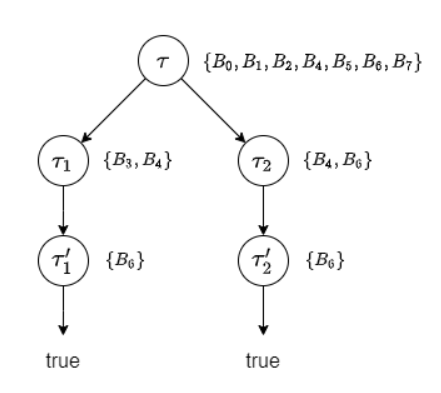
\includegraphics[width=0.5\textwidth,height=0.5\textwidth]{successful.png}
        \end{figure} \par
        \item Unsuccessful run. \par
        We guess a set $\tau = \{ B_0,B_3,  B_{10} \} \subseteq \operatorname{Def}_2$ with $B_0 \in \tau$. \\
        recurse$(\tau, 2, \mathcal{T})$: \\
        $\tau$ is not a type for $\mathcal{T}$ because $B_3 \in \tau, B_{10} \in \tau$ but $B_3 \equiv P$ and $B_{10} \equiv \lnot P$.
        Therefore, the algorithm return false.
        \newpage
        \begin{figure}[htbp]
            \centering 
            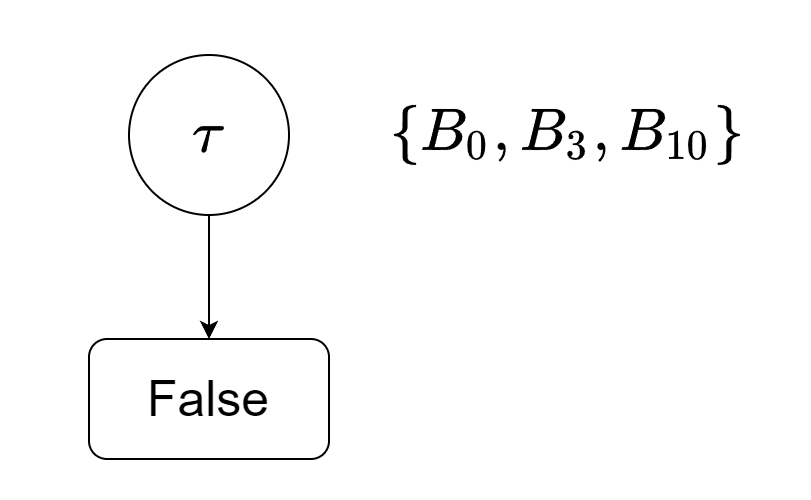
\includegraphics[width=0.5\textwidth,height=0.3\textwidth]{aaa.png}
        \end{figure} \par
    \end{itemize}
    Because there is a successful run, so the algorithm return a positive result.

    \newpage
    \paragraph{Question 2. Entailment Checking}~{}
    \\

    It holds true. \par
    For any model $ \mathcal{I} \models \{\forall r.A \sqsubseteq \exists r.A\} $, we'll prove that $ \mathcal{I} \models \{\forall r.B \sqsubseteq \exists r.B\} $ for all concept $B$.\par
    According to the semantics of $\mathcal{ALC}$:
    \begin{align*}
        \I & \models \{\forall r.A \sqsubseteq \exists r.A\} \\
        & \Rightarrow (\forall r.A)^{\mathcal{I}} \subseteq (\exists r.A)^{\mathcal{I}} 
    \end{align*} \par
    For a element $a \in \Delta^{\I}$, if there is no element $b$ such that $(a, b) \in r^{\I}$, then $a \in (\forall r.A)^{\I}$, so $a \in (\exists r.A)^{\I}$ due to $(\forall r.A)^{\mathcal{I}} \subseteq (\exists r.A)^{\mathcal{I}}$, obviously there is a contradiction. \par
    Therefore, $\forall a \in \Delta^{\I}$, there exist element $b \in \Delta^{\I}$ such that $(a, b) \in r^{\I}$. $\cdots$ (1)\par
    For a element $a$, if $a \in (\forall r.B)^{\I}$, then there at least exists a element $b$, such that $(a, b) \in r^{\I}$ and $b \in B^{\I}$, otherwise it contradicts conclusion (1), thus $a \in (\exists r.B)^{\I}$. \par
    Therefore, $(\forall r.B)^{\mathcal{I}} \subseteq (\exists r.B)^{\mathcal{I}}$, thus $ \mathcal{I} \models \{\forall r.B \sqsubseteq \exists r.B\} $.




    \newpage
    \paragraph{Question 3. Finite Boolean Games}~{}
    \\
    \begin{enumerate}
        \item [(1)]
        The figure following shows a winning strategy for Player 1 in G. 
        \begin{figure}[htbp]
            \centering 
            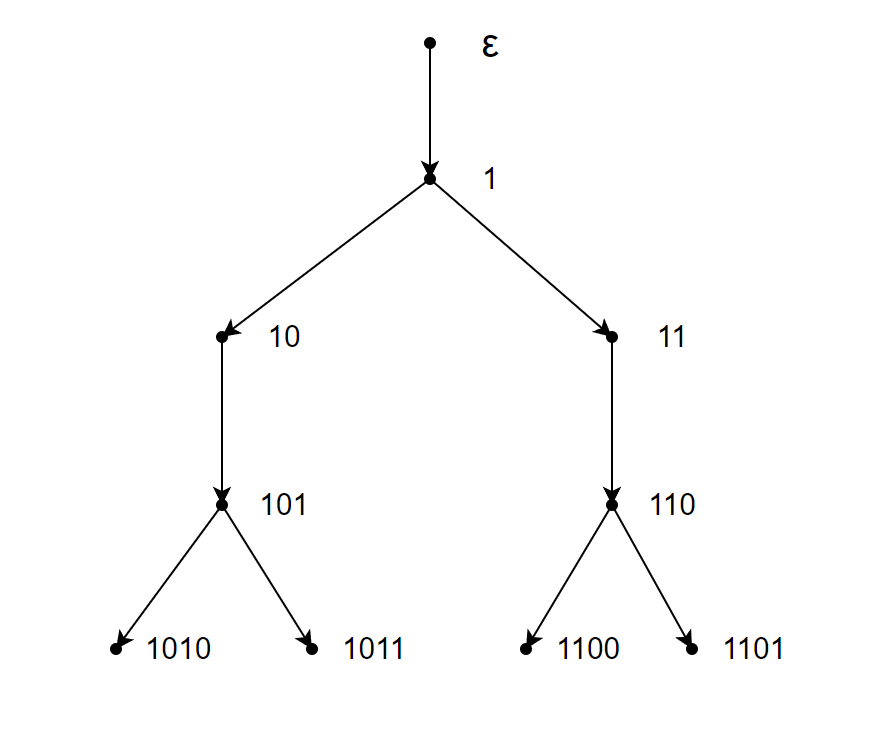
\includegraphics[width=0.5\textwidth,height=0.5\textwidth]{win1.png}
        \end{figure} \par
        \item [(2)]
        If Player 2 assign $x_2 = 0\ and\ x_4=1$, whatever Player1 do, there is no word t can satisfies $\varphi$. \\
        Therefore, Player 1 doesn't have a winning strategy.
    \end{enumerate}
    
    
    \newpage
    \paragraph{Question 4. Infnite Boolean Games}~{}
    \\
    
    \begin{enumerate}
        \item [(1)]
        Player 2 doesn't have a winning strategy. \\
        We can show that by showing Player 1 has a winning strategy.\\
        Player 1 assign $x_2 = 1$ and $x_3 = 1$ in the previous two turns.\\
        After assigning, $y_1 = 0$ or $y_2 = 0$, otherwise $(\lnot (x_1 \lor x_4) \land y_1 \land y_2) = 1$ and Player 1 wins.\\
        If $y_1 = \text{False}$, Player 1 can assign $x_1 = 1$ and then $(x_1 \land x_2 \land \lnot y_1) = 1$, so Player 1 wins.\\
        If $y_2 = \text{False}$, Player 1 can assign $x_4 = 1$ and then $(x_3 \land x_4 \land \lnot y_2) = 1$, so Player 1 wins. \\
        So Player 2 doesn't have a winning strategy.
        \item [(2)]
        Player 2 has a winning strategy. \\
        If $y_1 = 0, y_2 = 0$, the formule $\varphi$ is false, so Player 2 just need to assign 0 to $y_1$ and $y_2$ and he can win this game.
    \end{enumerate}

    \newpage
    \paragraph{Question 5. Complexity of Concept Satisfability in ALC Extensions}~{}
    \\

    Firstly we prove that concept satisfiability in $\mathcal{ALC}^{u}$ without TBoxes is EXPTIME-hard. $\cdots (1)$\par
    We have known in class that $\mathcal{ALC}$-concept satisfiability w.r.t. general TBox is EXPTIME-hard. So we need to prove that $\mathcal{ALC}$-concept satisfiability w.r.t. general TBox can be reduced to concept satisfiability in $\mathcal{ALC}^{u}$. \par
    Construct an $\mathcal{ALC}^{u}$-concept:
    $$
    D_0 = C_0 \sqcap \forall u.(\underset{C \sqsubseteq D \in \mathcal{T}}{\Large \sqcap} \lnot C \sqcup D)
    $$\par
    $C_0$ is satisfiable with respect to $\mathcal{T}$ iff $D_0$ is satisfiable with respect to $\mathcal{T}$. Now we prove it. \par
    $\Longleftarrow:$ \par
    Let $\mathcal{I}$ be a model of $D_0$, $d_0 \in D_0^{\mathcal{I}}$. \par
    Due to the universal rule, $\forall d \in D_0^{\mathcal{I}}$ we have $(d_0, d) \in u^{\mathcal{I}}$and therefore $d \in (\underset{C \sqsubseteq D \in \mathcal{T}}{\Large \sqcap} \lnot C \sqcup D)^{\mathcal{I}}$ ,which means $\forall d \in C^{\mathcal{I}}$ and $C \sqsubseteq D \in \mathcal{T}$, we have $d \in D^{\mathcal{I}}$ because $d \in (\lnot C \sqcup D)^{\mathcal{I}}$. \par
    So $\mathcal{I}$ is also a model of $C_0$ . \par
    $\Longrightarrow:$ \par
    Let $\mathcal{I}$ be a model of $C_0$ w.r.t. $\mathcal{T}$, $d_0 \in C_0^{\mathcal{I}}$. \par
    Modify $\mathcal{I}$ by setting $u^{\mathcal{I}}=\Delta^{\mathcal{I}} \times \Delta^{\mathcal{I}}$ . \par
    Since $C^{\mathcal{I}} \subseteq D^{\mathcal{I}}$ for all $C \sqsubseteq D \in \mathcal{T}$, we have $\Delta^{\mathcal{I}} \subseteq (\lnot C \sqcup D)^{\mathcal{I}}$ and therefore  $d_0 \in (\forall u.(\underset{C \sqsubseteq D \in \mathcal{T}}{\Large \sqcap} \lnot C \sqcup D))^{\mathcal{I}} = (\forall u.\top)^{\mathcal{I}} = \Delta^{\mathcal{I}}$.\par
    So $\mathcal{I}$ is also a model of $D_0$ . \par
    And now we have prove that the satisfiability of $\mathcal{ALC}$-concept $C_0$ can be reduced to the satisfiability of $\mathcal{ALC}^{u}$-concept $D_0$, thus concept satisfiability in $\mathcal{ALC}^{u}$ without TBoxes is EXPTIME-hard. \par
    Secondly, we prove that concept satisfiability in $\mathcal{ALC}^{u}$ without TBoxes has a EXPTIME upper bound. $\cdots (2)$\par
    We will modify $\mathcal{ALC}$-Elim algorithm to get $\mathcal{ALC}^{u}$-Elim algorithm, which is a EXPTIME algorithm.The only difference is the defnition of bad type:\par
    \begin{itemize}
        \item $\exists r.C \in \tau$  such that the set $S = \{C\} \cup \{ D| \forall r.D \in \tau \}$ is no subset of any type in $\Gamma$
        \item $\exists u.C \in \tau$ such that the set $S' = \{C\} \cup \{ D| \forall u.D \in \tau \}$ is no subset of any type in $\Gamma$
    \end{itemize} \par
    Now we prove that $\mathcal{ALC}^{u}$-Elim$(A_0, \mathcal{T} )$ returns 'true' iff $A_0$ is satisfifiable w.r.t. $\mathcal{T}$.\par
    $\Longrightarrow:$ \par
    Construct a model $\mathcal{I}$ use the result of $\mathcal{ALC}^{u}$-Elim$(A_0, \mathcal{T} )$ :\par
    $$
    \begin{aligned}\Delta^{\mathcal{I}} &= \Gamma_i\\
    A^{\mathcal{I}} &= \{{ \tau \in \Gamma_i | A \in \tau \}}\\
    r^{\mathcal{I}} &= \{{ (\tau, \tau') \in \Gamma_i \times \Gamma_i | \forall r.C \in \tau \text{ implies } C \in \tau' }\}\end{aligned}
    $$
    \begin{itemize}
        \item Let $\exists u.D \in \tau$. Since $\tau$ has not been eliminated from $\Gamma_i$, it is not bad. Thus, there is a $\tau' \in \Gamma$, such that $\{ D \} \subseteq \tau'$. Because we have $(\tau'', \tau') \in u^{\mathcal{I}}$ for any type $\tau''$, we obtain $\tau'' \in (\exists r.D)^{\mathcal{I}}$ by the semantics, and it also includes $\tau \in (\exists r.D)^{\mathcal{I}}$.
        \item Let $\forall u.D \in \tau$. Since $\tau$ has not been eliminated from $\Gamma_i$, it is not bad. Thus, there is $D \in \tau'$ for all type $\tau'$, we obtain $\tau' \in D^{\mathcal{I}}$ and $\tau' \in (\forall u.D)^{\mathcal{I}}$ by the semantics, and it also include $\tau \in D$ and $\tau \in (\forall u.D)^{\mathcal{I}}$.
    \end{itemize} \par
    $\Longleftarrow:$ \par
    If  $A_{0} $ is satisfiable with respect to  $\mathcal{T}$ , then there is a model $ \mathcal{I}$  of $ A_{0}$  and  $\mathcal{T}$ . Let $ d_{0} \in A_{0}^{\mathcal{I}} $. For all $d \in \Delta^{\mathcal{I}}$, 
    $$
    \operatorname{tp}(d) = \{ C \in \operatorname{sub}(\mathcal{T}) | d \in C^{\mathcal{I}} \}
    $$ \par
    Define $\Psi = \{ \operatorname{tp}(d) | d \in \Delta^{\mathcal{I}} \}$ and let  $\Gamma_0, \Gamma_1, \cdots, \Gamma_{k}$ be the sequence of type sets computed by $\mathcal{ALC}^{u}$-Elim$(A_0, \mathcal{T})$. It is possible to prove by induction on $i$ that no type from $\Psi$ is ever eliminated from any set $\Gamma_i$, for $i \le k$. So the algorithm return "true". \par

    According to the conclusion (1) and (2), we can get that concept satisfability in $\mathcal{ALC}^{u}$ without TBoxes is EXPTIME-complete.

    \newpage
    \paragraph{Question 6. Conservative Extension}~{}
    \\

    \begin{enumerate}
        \item [(1)]
        $\because sig(\T_2) = sig(\T_1) \cup \{A,B\}\quad \therefore sig(\T_1) \subseteq sig(\T_2)$ \par
        $\because \T_1 \subseteq \T_2 \quad \therefore \text{ every model of }\T_2 \text{ is a model of } \T_1$ \par
        For every model $\I_1$ of $\T_1$, we can construct a model $\I_2$ as follow: \par
        \begin{itemize}
            \item $\Delta^{\I_2} = \Delta^{\I_1}$
            \item $E^{\I_2} = E^{\I_1}$ for all concept names $E$ in $\T_1$, $A^{\I_2} = C^{\I_1}, B^{\I_2} = D^{\I_1}$
            \item $r^{\I_2} = r^{\I_1}$ for all roles in $\T_1$
        \end{itemize}
        Obviously, $\I_2$ is a model of $\T_2$ and the extensions of concept and role names from $sig(\T_1)$ coincide in $\I_1$ and
        $\I_2$. \par
        Therefore, $\T_2$ is a conservative extension of $\T_1$.
        \item [(2)]
        After adding $A \sqsubseteq B$, it still holds. \par
        The only difference of the model $\I_2$ we construct with (1) is:
        $A^{\I} = \emptyset$. \par
        We can get that $A^{\I} \subseteq B^{\I}$ so $\I_2$ is still a model of $\T_2$ and the extensions of concept and role names from $sig(\T_1)$ coincide in $\I_1$ and
        $\I_2$. \par
        Therefore, $\T_2$ is a conservative extension of $\T_1$.
        \item [(3)]
        It dose not hold. \par
        After adding $B \sqsubseteq A$, we can get that $D \sqsubseteq C$ in $\T_2$. \par
        For some model $\I_1$ w.r.t. $\T_1$, if there exists element $a \in \Delta^{\I_1}$ such that $a \in D^{\I_1}$ but $a \not\in C ^{\I_1}$, then it is impossible to find a model $\I_2$ w.r.t. $\T_2$ and the extensions of concept and role names from $sig(\T_1)$ coincide in $\I_1$ and $\I_2$. (because there exists $D^{\I_1} \neq D^{\I_2}$ or $C^{\I_1} \neq C^{\I_2}$)
    \end{enumerate}
    
        

    \newpage
    \paragraph{Question 7. Subsumption in $\mathcal{EL}$}~{}
    \\

    Normalization TBox $\T$: 
    \begin{align*}
        A \sqsubseteq B \sqcap \exists r.C & \rightarrow_{NF4} A \sqsubseteq B, A \sqsubseteq \exists r.C\\
        B \sqcap \exists r.B \sqsubseteq C \sqcap D &\rightarrow_{NF0} \underline{B \sqcap \exists r.B \sqsubseteq E_0}, \underline{E_0 \sqsubseteq C \sqcap D}\\
        B\sqcap\exists r.B\sqsubseteq E_0 & \rightarrow_{NF1_r} \exists r.B\sqsubseteq E_1,B\sqcap E_1\sqsubseteq E_0 \\
        E_0 \sqsubseteq C \sqcap D & \rightarrow_{NF4} E_0 \sqsubseteq C, E_0 \sqsubseteq D \\
        C\sqsubseteq(\exists r.A)\sqcap B & \rightarrow_{NF4} C\sqsubseteq\exists r.A,C\sqsubseteq B \\
        (\exists r.\exists r.B)\sqcap D\sqsubseteq\exists r.(A\sqcap B)&\rightarrow_{NF0} \underline{(\exists r.\exists r.B)\sqcap D\sqsubseteq E_2}, \underline{E_2\sqsubseteq\exists r.(A\sqcap B)} \\
        (\exists r.\exists r.B)\sqcap D\sqsubseteq E_2 & \rightarrow_{NF1_l} \underline{(\exists r.\exists r.B)\sqsubseteq E_3},E_3\sqcap D\sqsubseteq E_2 \\
        (\exists r.\exists r.B)\sqsubseteq E_3 & \rightarrow_{NF2} \exists r.B\sqsubseteq E_4,\exists r.E_4\sqsubseteq E_3 \\
        E_2\sqsubseteq\exists r.(A\sqcap B) & \rightarrow_{NF3} \underline{E_5\sqsubseteq A\sqcap B}, E_2\sqsubseteq\exists r.E_5 \\
        E_5\sqsubseteq A\sqcap B &\rightarrow_{NF4} E_5\sqsubseteq A,E_5\sqsubseteq B 
    \end{align*} \par
    We get the normalised TBox $\T' = \{A\sqsubseteq B,A\sqsubseteq\exists r.C,\exists r.B\sqsubseteq E_1,B\sqcap E_1\sqsubseteq E_0,E_0\sqsubseteq C,E_0\sqsubseteq D,C\sqsubseteq\exists r.A,C\sqsubseteq  B,E_3\sqcap D\sqsubseteq E_2,\exists r.B\sqsubseteq E_4,\exists r.E_4\sqsubseteq E_3,E_2\sqsubseteq\exists r.E_5,E_5\sqsubseteq A,E_5\sqsubseteq B\}$
    \begin{enumerate}
        \item [(1)]
        $A \sqsubseteq B$ already exists in $\T'$, so it holds w.r.t. to $\T^{\prime}$.
        \item [(2)]
        According to lemma 6.1, $\mathcal{T} \models A \sqsubseteq \exists r . \exists r . A \text{ iff }
        \mathcal{T} \cup\{F \sqsubseteq A, \exists r . \exists r . A \sqsubseteq G\} \models F \sqsubseteq G$. Normalization $\mathcal{T} \cup\{F \sqsubseteq A, \exists r . \exists r . A \sqsubseteq G\}$, we get $\T^{\prime\prime} = \T' \cup \{F \sqsubseteq A, \exists r.A \sqsubseteq H, \exists r.H \sqsubseteq G\}$ 
        \begin{align*}
            &\text{ Apply CR3 to } C \sqsubseteq \exists r.A, \exists r.A \sqsubseteq H \rightarrow C \sqsubseteq H \\
            &\text{ Apply CR3 to } F \sqsubseteq A, A \sqsubseteq \exists r.C\rightarrow F \sqsubseteq \exists r.C \\
            &\text{ Apply CR5 to } F \sqsubseteq \exists r.C, C \sqsubseteq H, \exists r.H \sqsubseteq G \rightarrow  F \sqsubseteq G \\
        \end{align*}
    we have $F \sqsubseteq G$, so $A \sqsubseteq \exists r.\exists r.A$ holds.\\
    \item [(3)]
    We can get $\T^{\prime\prime} = \T' \cup \{F \sqsubseteq B, F \sqsubseteq \exists r.A, \exists r.C \sqsubseteq G\}$ just like (2).
    \begin{align*}
        &\text{ Apply CR5 to } A \sqsubseteq \exists r.C, C \sqsubseteq B, \exists r.B \sqsubseteq E_1 \rightarrow A \sqsubseteq E_1 \\
        &\text{ Apply CR3 to } B \sqcap E_1 \sqsubseteq E_0, E_0 \sqsubseteq C \rightarrow B \sqcap E_1 \sqsubseteq C \\
        &\text{ Apply CR4 to } A \sqsubseteq B, A \sqsubseteq E_1, B \sqcap E_1 \sqsubseteq C \rightarrow  A \sqsubseteq C \\
        &\text{ Apply CR5 to } F \sqsubseteq \exists r.A, A \sqsubseteq C, \exists r.C \sqsubseteq G \rightarrow F \sqsubseteq G 
    \end{align*}
    we have $F \sqsubseteq G$, so $B \sqcap \exists r.A \sqsubseteq \exists r.C$ holds.\\
    \end{enumerate}

    \newpage
    \paragraph{Question 8. Simulation}~{}
    \\

    \begin{enumerate}
        \item [(a)]
        According to the defnition of bisimulation $(\I,d) \sim (\J,d')$: \par
        \begin{enumerate}
            \item [(i)] $d\rho d'$ implies $d \in A^{\I}$ $\Leftrightarrow$ $d' \in A^{\J}$ for all $A \in \mathbb{C}$.
            \item [(ii)] $d\rho d'$ and $(d,e) \in r^{\I}$ implies there exists $e' \in \Delta^{\J}$ so that $e\rho e'$ and $(d',e') \in r^{\J}$.
            \item [(iii)] $d\rho d'$ and $(d',e') \in r^{\J}$ implies there exists $e \in \Delta^{\I}$ so that $e\rho e'$ and $(d,e) \in r^{\I}$.
        \end{enumerate}
        We can get $(\I,d) \eqsim (\J,d')$ because of (i) and (ii), $(\J,d') \eqsim (\I,d)$ because of (i) and (iii).
        \item [(b)]
        Here is the counterexample: \par
        \begin{figure}[htbp]
            \centering 
            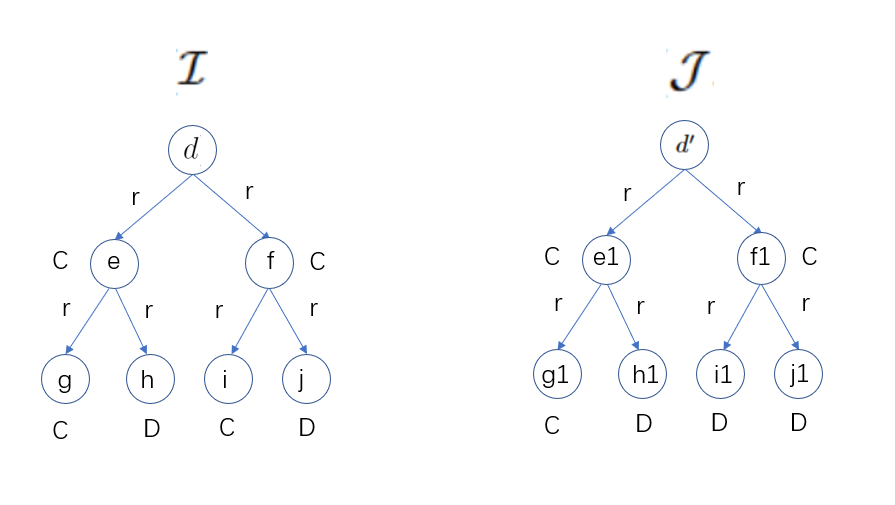
\includegraphics[width=0.8\textwidth,height=0.5\textwidth]{HW8_B.png}
        \end{figure} \par
        We can get $(\I,e) \eqsim (\J,e1)$ and $(\I,f) \eqsim (\J, f1)$ so
        $(\I,d) \eqsim (\J,d')$. \par
        We can get $(\J,e1) \eqsim (\I, f)$ and $(\J, f1) \eqsim (\I, f)$ so $(\J,d') \eqsim (\I,d)$. \par
        But obviously $ (\mathcal{I}, d) \not\sim (\mathcal{J}, d') $
        \item [(c)]
        \begin{itemize}
            \item Assume $C = A \in \mathbf{C}$(Concept name). 
            $$d \in C^{\I} \text{ implies }d' \in C^{J}$$ is an immediate consequence due to the defnition of $ (\mathcal{I}, d) \sim (\mathcal{J}, d') $
            \item Assume $C=\top$.
            $$d \in C^{\I} \text{ implies }d' \in C^{J}$$ is an immediate consequence due to the defnition of $ (\mathcal{I}, d) \sim (\mathcal{J}, d') $
            \item Assume $C = D \sqcap E$. \\
            If $d\in C^{\mathcal{I}}$ then $d\in D^{\mathcal{I}}\cap E^{\mathcal{I}}$ implies $d\in D^{\mathcal{I}},d\in E^{\mathcal{I}},$ which implies
            $d'\in D^{\mathcal{J}},d'\in E^{\mathcal{J}},d'\in(D\sqcap E)^{\mathcal{J}}=C^{\mathcal{J}}$.
            \item Assume $C=\exists r.D$. \\
            If $d \in C^\mathcal{I}$ then there exists an $e \in D^\mathcal{I}$ and $(d,e)\in r^\mathcal{I}$, which implies there exists an $e' \in D^{\mathcal{J}},(d',e') \in r^{\mathcal{J}}$. So $d' \in C^{\J}$. 
        \end{itemize}
        \item [(d)]
        For disjunction: \par
        Assume $C = D \sqcup E$. If $ d \in C^{\mathcal{I}} $, 
        then we have $ d \in D^{\mathcal{I}} $ or $ d \in E^{\mathcal{I}} $. We have $ d' \in D^{\mathcal{J}} $ or $ d' \in E^{\mathcal{J}} $.
        So we have $ d' \in (D \sqcup E)^{\mathcal{J}} = C^{\J} $ \par
        Therefore, disjunction can be added to $\mathcal{EL}$ without losing the property in (c).
        For negation: \par
        Let $ A^{\mathcal{I}} = \{e\}, \Delta^{\mathcal{I}} = \{d, e\} $ 
        and $ A^{\mathcal{J}} = \{d'\}, \Delta^{\mathcal{J}} = \{d', e'\} $.
        We have $ (\mathcal{I}, d) \eqsim (\mathcal{J}, d') $ and 
        $ d \in (\neg A)^{\mathcal{I}} $.
        But $ d' \notin (\neg A)^{\mathcal{J}}$. \par
        Therefore, negation can not be added without lose the property. \par
        For value restriction: \par
        Let $ A^{\mathcal{I}} = \{a\}, r^{\mathcal{I}} = \emptyset, \Delta^{\mathcal{I}} = \{a, b\} $ 
        and $ A^{\mathcal{J}} = \{a'\}, r^{\mathcal{J}} = \{(a',b')\}, \Delta^{\mathcal{J}} = \{a', b'\} $.
        We have $ (\mathcal{I}, a) \eqsim (\mathcal{J}, a') $ and 
        $ a \in (\forall r.A)^{\mathcal{I}} $.
        But  $ a' \notin (\forall r.A)^{\mathcal{J}}$.\\
        Therefore, value restriction can not be added without lose the property. \par
        \item [(e)]
        The above consequence in (c) states that $\mathcal{EL}$ cannot distinguish between simulate elements. But $\mathcal{ALC}$ can. Look at the example as follow: \par
        $\Delta^{\I} = \{a,b,c\},A^{\I} = \{a, b\},B^{\I} = \{c\}$\\
        $\Delta^{\J} = \{a',b',c'\},A^{\I} = \{a', b', c'\},B^{\I} = \{c'\}$\\
        Obviously, $(\I,c) \eqsim (\J, c')$. But $c \in (\neg A)^{\I}$ while $c' \not \in (\neg A)^{\J}$\\
        So $\ALC$ is more expressive than $\mathcal{EL}$\\
    \end{enumerate}


    \newpage
    \paragraph{Question 9. $\mathcal{EL}$ Extension}~{}
    \\
    \begin{enumerate}
        \item [(1)]

To show that each $\mathcal{EL}$si concept description is equivalent to some concept descriptions of the form $\exists \text{sim}(I, d)$, we need to demonstrate that any $\mathcal{EL}$si concept description can be represented using $\exists \text{sim}(I, d)$ and vice versa.

Let's start with an $\mathcal{EL}$si concept description of the form $\exists \text{sim}(I, \delta)$, where $I$ is a finite interpretation and $\delta \in \Delta^I$. We want to show its equivalence to a concept description of the form $\exists \text{sim}(I, d)$.

To do this, we'll represent $\delta$ as a concept description using $\exists \text{sim}(I, d)$. Consider the concept description $\delta' = \{x \mid \exists \text{sim}(I, \delta)(x)\}$.

Now, let's analyze the semantics of both descriptions:

\begin{itemize}
  \item $(\exists \text{sim}(I, \delta))J$: This represents the set of individuals in the interpretation $J$ that satisfy the concept description $\exists \text{sim}(I, \delta)$. In other words, it includes individuals in $J$ for which there exists an individual in $I$ that is similar to them according to $\delta$.

  \item $(\exists \text{sim}(I, d))J$: This represents the set of individuals in the interpretation $J$ that satisfy the concept description $\exists \text{sim}(I, d)$. Similarly, it includes individuals in $J$ for which there exists an individual in $I$ that is similar to them according to $d$.
\end{itemize}

We need to show that $(\exists \text{sim}(I, \delta))J = (\exists \text{sim}(I, d))J$. To prove this, we'll demonstrate that $(\exists \text{sim}(I, \delta))J \subseteq (\exists \text{sim}(I, d))J$ and $(\exists \text{sim}(I, d))J \subseteq (\exists \text{sim}(I, \delta))J$.

\begin{enumerate}
  \item $(\exists \text{sim}(I, \delta))J \subseteq (\exists \text{sim}(I, d))J$: Let's assume an individual $a \in (\exists \text{sim}(I, \delta))J$. It means that there exists an individual $b$ in $I$ such that $(I, \delta)$ is similar to $(J, a)$. Since $\delta'$ represents $\exists \text{sim}(I, \delta)$, we can say that $b \in (\exists \text{sim}(I, d))J$, as $(I, d)$ is similar to $(J, a)$. Therefore, $(\exists \text{sim}(I, \delta))J \subseteq (\exists \text{sim}(I, d))J$.

  \item $(\exists \text{sim}(I, d))J \subseteq (\exists \text{sim}(I, \delta))J$: Assume an individual $c \in (\exists \text{sim}(I, d))J$. It implies that there exists an individual $d$ in $I$ such that $(I, d)$ is similar to $(J, c)$. Since $\delta$ represents $\exists \text{sim}(I, \delta)$, we can say that $d \in (\exists \text{sim}(I, \delta))J$, as $(I, \delta)$ is similar to $(J, c)$. Hence, $(\exists \text{sim}(I, d))J \subseteq (\exists \text{sim}(I, \delta))J$.
\end{enumerate}

Therefore, we have shown that $(\exists \text{sim}(I, \delta))J = (\exists \text{sim}(I, d))J$. This demonstrates the equivalence between the $\mathcal{EL}$si concept description $\exists \text{sim}(I, \delta)$ and the concept description $\exists \text{sim}(I, d)$.

By extension, we can conclude that any ELsi concept description can be represented by a concept description of the form $\exists \text{sim}(I, d)$, and vice versa.


        \item [(2)]
        Construct interpretation $\I$: 
        \begin{align*}
            \Delta^{\mathcal{I}} &= \{d\} \\
            A^\mathcal{I} &= \{d\} \text{ for each } A \in \mathbb{C}
        \end{align*}\par
        However, there are no roles in $ \mathcal{I} $. Consequently, any element simulated by $ d $ must belong to the extensions of all concepts $ A\in\mathbb{C} $. The concept $ \exists^{\rm sim}(\mathcal{I}, d) $ is equivalent to $ \prod\limits_{A\in\mathbb{C}}A $.

Now let's prove that no $ \mathcal{EL} $ concept is equivalent to $ \exists^{\rm sim}(\mathcal{I}, d) $. Consider any concept $ C $ that is not the intersection of all concept names. There must exist a concept name $ A \notin {\rm sub}(C) $. \\
We can construct a model $ \mathcal{J} $ as follows: \\
$r^{\mathcal{J}}$ is empty for all role names in $ C $. \\
$A^{\mathcal{J}} = \left\{\begin{array}{ll}
\{a, b\} & A\in {\rm sub}(C)\\
\{a\} & A \not \in {\rm sub}(C)
\end{array}\right. $ for all concept names $ A \in \mathbb{C} $. \\
$ \Delta^{\mathcal{J}} = \{a, b\} $. \\
In this model, any concepts of the form $ \exists r.E $ will be interpreted as $ \emptyset $ by $ \mathcal{J} $. Consequently, any concepts in $ {\rm sub}(C) $ will be interpreted as $ \emptyset $ or $ {a, b} $ by $ \mathcal{J} $. However, $ (\exists^{\rm sim}(\mathcal{I}, d))^{\mathcal{J}} = { a } $. Thus, no $ \mathcal{EL} $ concept is equivalent to the $ \mathcal{EL}_{\rm si} $ concept.

Therefore, $ \mathcal{EL}_{\rm si} $ is more expressive than $ \mathcal{EL} $.
        \item [(3)]
        To show that checking subsumption in $\mathcal{EL}$si without any TBox can be done in polynomial time, we need to demonstrate that there exists a polynomial-time algorithm that can determine whether one $\mathcal{EL}$si concept is a subsumed by another $\mathcal{EL}$si concept.

Given two $\mathcal{EL}$si concepts, $C_1$ and $C_2$, the algorithm for checking subsumption can proceed as follows:

1. If $C_1$ is equivalent to $C_2$, return true. \\
2. If $C_1$ is of the form $\exists^{\text{sim}}(I_1, d_1)$ and $C_2$ is of the form $\exists^{\text{sim}}(I_2, d_2)$, check if $I_1$ and $I_2$ have a non-empty intersection. If they do and $d_1 = d_2$, return true. Otherwise, return false. \\
3. If $C_1$ is of the form $\exists^{\text{sim}}(I_1, d_1)$ and $C_2$ is of the form $D_2$, recursively check if $D_2$ subsumes $\exists^{\text{sim}}(I_1, d_1)$. If it does, return true. Otherwise, return false. \\
4. If $C_1$ is of the form $D_1$ and $C_2$ is of the form $\exists^{\text{sim}}(I_2, d_2)$, return false. \\
5. If $C_1$ is of the form $D_1$ and $C_2$ is of the form $D_2$, recursively check if $D_1$ subsumes $D_2$. If it does, return true. Otherwise, return false. \\
This algorithm checks each possible case and terminates in a finite number of steps. The size of the input concepts and interpretations can be represented using polynomially bounded space. Thus, the algorithm runs in polynomial time.

Therefore, checking subsumption in $\mathcal{EL}$si without any TBox can be done in polynomial time.
    \end{enumerate}



    \newpage
    \paragraph{Question 10 (with 1 bonus mark). $\mathcal{ALC}$-Elim Algorithm}~{}
    \\

    \begin{enumerate}
        \item [(1)]
        We firstly caculate $C_{\T}$ and $sub(\T)$:
        \begin{align*}
            C_{\T} &= A \sqcap(\neg A \sqcup \exists r. A) \sqcap (\exists r.\neg A \sqcup \exists r.A) \\
            sub(\T) &= \{\exists r.\neg A, \neg A,\exists r.A, \exists r.\neg A\sqcup \exists r.A, \neg A \sqcup \exists r.A, A, A \sqcap(\exists r.\neg A \sqcup \exists r. A),C_{\T}\}
        \end{align*} \par
        Then we run $\ALC-Elim$ algorithm. \par
        $\ALC-Elim(A,\T)$: \par
        \quad loop:

        \qquad $i=0$ \par
        \qquad $\varGamma_0=\{\tau_1,\tau_2\}$ \par
        \qquad $\tau_1 =\{\exists r.A, \exists r.\neg A\sqcup \exists r.A, \neg A \sqcup \exists r.A, A, A \sqcap(\exists r.\neg A \sqcup \exists r. A),C_{\T}\}$ \par
        \qquad i=1:

    \qquad $S = \{A\} \subseteq \tau_1$, $\tau_1$ is not bad

    \qquad $S = \{\neg A\} \not \subseteq \tau_1$ or $\tau_2$, $\tau_2$ is bad!

    \qquad $\varGamma_1 = \{\tau_1\}$

    \qquad $i=2,\varGamma_2 = \varGamma_1 = \{\tau_1\}$, break the loop! 
    
    \quad $A \in \tau_1$,\quad return true \par
    The satisfying model $\I$: 
    \begin{align*}
        \Delta^{\I} &= \{\tau_1\} \\
        A^{\I} &= \{\tau_1\} \\
        r^{\I} &= \{(\tau_1,\tau_1)\}
    \end{align*}
        \item [(2)]
        Add $D \sqsubseteq \forall r.\forall r.\neg B$ to $\T$, where $D$ is a fresh concept name. \par
        We firstly caculate $C_{\T}$, $sub(\T)$ and $\tau_i$:
        \begin{align*}
            C_{\T} &= (\neg A \sqcup \neg B)\sqcap (A \sqcup B) \sqcap \exists r.\neg A \sqcap(\neg D \sqcup \forall r.\forall r.\neg B) \\
            sub(\T) &= \{\forall r.\neg B,\forall r.\forall r.\neg B,D,\neg D, A,\neg A,B,\neg B, \neg C \sqcup \forall r.\forall r.\neg B,\exists r.\neg A, \neg A \sqcup \neg B, \\ & A \sqcup B, (A \sqcup B)\sqcap (\neg A \sqcup \neg B), (A \sqcup B)\sqcap (\neg A \sqcup \neg B) \sqcap \exists r.\neg A, C_{\T}\} \\
            \tau_0 &= \{\neg C \sqcup \forall r.\forall r.\neg B,\exists r.\neg A, \neg A \sqcup \neg B, A \sqcup B, (A \sqcup B)\sqcap (\neg A \sqcup \neg B), \\ & (A \sqcup B)\sqcap (\neg A \sqcup \neg B) \sqcap \exists r.\neg A, C_{\T}\}
        \end{align*}
        \qquad $\tau_1 = \tau_0 \cup \{A,\neg B,\neg D\}$ \qquad $\tau_2 = \tau_1 \cup \{\forall r.\neg B\}$ \qquad $\tau_3 = \tau_0 \cup \{A,\neg B,\forall r.\forall r.\neg B\}$

    \qquad $\tau_4 = \tau_3 \cup \{D\}$ \qquad $\tau_5 = \tau_3 \cup \{\forall r.\neg B\}$ \qquad $\tau_6 = \tau_3 \cup \{\forall r.\neg B,D\}$

    \qquad $\tau_7 = \tau_3 \cup \{\neg D\}$ \qquad $\tau_8 = \tau_3 \cup \{\neg D,\forall r.\neg B\}$ \qquad $\tau_9 = \tau_0 \cup \{\neg A, B,\neg D\}$

    \qquad $\tau_{10} = \tau_9 \cup \{\forall r.\neg B\}$ \qquad $\tau_{11} = \tau_0 \cup \{\neg A, B,\forall r.\forall r.\neg B\}$ \qquad $\tau_{12} = \tau_{11} \cup \{D\}$

    \qquad $\tau_{13} = \tau_{11} \cup \{\forall r.\neg B\}$ \qquad $\tau_{14} = \tau_{11} \cup \{D,\forall r.\neg B\}$ \qquad $\tau_{15} = \tau_{11} \cup \{\neg D\}$

    \qquad $\tau_{16} = \tau_{11} \cup \{\neg D,\forall r.\neg B\}$ \par
        Then we run $\ALC-Elim$ algorithm. \par
        $\ALC-Elim(A,\T)$: \par
        \quad loop: 

        \qquad $i=0$, $\varGamma_0=\{\tau_i|i\in [16]\}$

        \qquad $i=1$, $\tau_2,\tau_5,\tau_6,\tau_8,\tau_{10},\tau_{13},\tau_{14},\tau_{16}$ are bad.

    \qquad $\varGamma_1=\{\tau_1,\tau_3,\tau_4,\tau_7,\tau_9,\tau_{11},\tau_{12},\tau_{15}\}$

    \qquad $i=2:$, $\tau_3,\tau_4,\tau_7,\tau_{11},\tau_{12},\tau_{15}$ are bad.

    \qquad $\varGamma_2 = \{\tau_1,\tau_9\}$

    \qquad $i=3:$

    \qquad $\varGamma_3 = \varGamma_2 $, break the loop!
    
    \quad $D \not \in \tau_1$ or $\tau_9$,\quad return false \par
    
    Therefore, $\forall r.\forall r.\neg B$ is not satisfiable w.r.t $\T$. 
    \end{enumerate}
    

    \newpage
    \paragraph{Question 11 (with 1 bonus mark). $\mathcal{ALCI}$-Elim algorithm}~{}
    \\
    
    Extend definition 5.9 in text book: \par
    Let $\varGamma$ be a set of types and $\tau \in \varGamma$. Then $\tau$ is bad in $\varGamma$ if: \par
    1. there exists an $\exists r.C \in \tau$ such that the set$$ S = {C} \cup \{D|\forall r.D \in \tau \}$$ \par is no subset of any type in $\varGamma$.  \par
    or \par
    2. there exists an $\exists r^{-}.C \in \tau$ such that the set $$ S = {C} \cup \{D|\forall r^{-}.D \in \tau \}$$ \par is no subset of any type in $\varGamma$. \par
    The rest of the process is the same as in the textbook. \par
    Prove of correctness(based on lemma 5.10 in text book): \par
    Assume that $\mathcal{ALC}$-Elim($\A_0, \T$) returns true, and let $\varGamma_i$ be the set of remaining types. Then there is a $\tau_o \in \varGamma_i$ such that $\A_0 \in \tau_0$. \par
    Define an interpretation I as follows: 
    \begin{align*}
        \Delta^{\I} & = \varGamma_i\\
        A^{\I} & = \{ \tau \in \varGamma_i | A \in \tau \} \\
        r^{\I} & = \{(\tau,\tau') \in \varGamma_i \times \varGamma_i | \forall r.C \in \tau \quad \text{implies} \quad C \in \tau'\}
    \end{align*} \par
    By induction on the structure of $C$, we can prove, for all $C \in sub(\T)$ and all $\tau \in \varGamma_i$, that $C \in \tau$ implies $\tau \in C^{\I}$. Most cases are straightforward, using the definition of $\I$ and the induction hypothesis. We only do the case $C = \exists r. D$, $C = \exists r^{-}.D$ and $C = \forall r^{-}.D$ explicitly: \par
    \begin{itemize}
        \item Let $\exists r.D \in \tau$. Since $\tau$ has not been eliminated from $\varGamma_i$, it is not bad.
        Thus, there is a $\tau^{\prime} \in \varGamma_i$ such that
        $$\{C\} \cup\{D \mid \forall r . D \in \tau\} \subseteq \tau^{\prime}.$$ \par
        By definition of $\I$, we have $(\tau, \tau^{\prime}) \in r^{\I}$. Since $\tau^{\prime} \in C^{\I}$ by induction hypothesis, we obtain $\tau \in (\exists r.C)^{\I}$ by the semantics.
        \item let $\exists r^{-}.D \in \tau$. Since $\tau$ has not been eliminated from $\varGamma_i$, it is not bad.
        Thus, there is a $\tau' \in \varGamma_i$ such that $$\{D\} \cup \{E | \forall r^{-}.E \in \tau\} \subseteq \tau'$$\par
        If there exists $\forall r.E \in \tau'$, then $E \in \tau$ because $\tau'$ is not bad, and thus $(\tau',\tau) \in r^{\I}$.We obtain $\tau \in (\exists r^{-}.D)^{\I}$ by the semantics.
        \item Let $\forall r^{-}.D \in \tau$. Since $\tau$ has not been eliminated from $\varGamma_i$, it is not bad. If there is a $\tau' \in \varGamma_i$ and $(\tau',\tau) \in r^{\I}$, then $D \in \tau'$.\\
        So $\tau' \in D^{\I}$, we obtain $\tau \in (\forall r^{-}.D)^{\I}$ by semantics. \par
        Hence, $\I$ is a model of $\T$. Since $\A_0 \in \tau_0$, it is also a model of $\A_0$.
    \end{itemize}

    \newpage
    \paragraph{Question 12 (with 1 bonus mark). Subsumption in $\mathcal{ELI}$}~{}
    \\

    Normalization the TBox and get $$\T^{\prime} = \{\{A_1,A_2\}\sqsubseteq \exists r.\{B\},\{A_2\}\sqsubseteq \forall r.\{C\},\{A\} \sqsubseteq\{A_1,A_2\},\{B,C\}\sqsubseteq \forall r^{-}.\{D\}\}$$
    \begin{enumerate}
        \item [(1)]
        \begin{align*}
            &\text{Apply CR1:}\{A_1,A_2\}\sqsubseteq\{A_2\} \\
            &\text{Apply CR2:}\{A\}\sqsubseteq\{A_1,A_2\},\{A_1,A_2\}\sqsubseteq\{A_2\}\to\{A\}\sqsubseteq\{A_2\} \\
            &\text{Apply CR2:}\{A\}\sqsubseteq\{A_1,A_2\},\{A_1,A_2\}\sqsubseteq\exists r.\{B\}\to\{A\}\sqsubseteq\exists r.\{B\} \\
            &\text{Apply CR2:}\{A\}\sqsubseteq\{A_2\},\{A_2\}\sqsubseteq\forall r.\{C\}\to\{A\}\sqsubseteq\forall r.\{C\} \\
            &\text{Apply CR4:}\{A\}\sqsubseteq\forall r.\{C\},\{A\}\sqsubseteq\exists r.\{B\}\to\{A\}\sqsubseteq\exists r.\{B,C\} \\
            &\text{Apply CR3:}\{A\}\sqsubseteq\exists r.\{B,C\},\{B,C\}\sqsubseteq\forall r^{-}.\{D\}\to\{A\}\sqsubseteq\{D\}
            \end{align*} \par
        We have $\{A\} \sqsubseteq \{D\}$, so $A \sqsubseteq D$ holds.
        \item [(2)]
        According to lemma 6.1(just like Question 8(2)), we can get $$\T^{\prime\prime} = \T' \cup\{\{E\} \sqsubseteq \exists r.\{A\},\{D\} \sqsubseteq \forall r^{-}.\{F\}\}$$
        \begin{align*}
            &\text{Apply CR2:}\{A\}\sqsubseteq\{D\},\{D\}\sqsubseteq \forall r^{-}.\{F\} \to \{A\} \sqsubseteq \forall r^{-}.\{F\} \\
            &\text{Apply CR3:}\{E\}\sqsubseteq \exists r.\{A\},\{A\}\sqsubseteq \forall r^{-}.\{F\}\to\{E\}\sqsubseteq\{F\} 
        \end{align*}   \par
        We have $\{E\}\sqsubseteq\{F\}$, so $\exists r . A \sqsubseteq \exists r . D$ holds.
        \item [(3)]
        If we want to get $\{A\} \sqsubseteq \exists r.\{A\}$, we must apply CR4 to some $M_{1} \sqsubseteq \exists r. M_{2} , M_{1} \sqsubseteq \forall r .\{A\}$, there is no CR4-rule could apply to get $\{A\} \sqsubseteq \exists r.\{A\}$ and there isn't $\{A\} \sqsubseteq \exists r.\{A\}$, so we can conclude that $A \sqsubseteq \exists r . A$ doesn't hold.
    \end{enumerate}
\end{document}
